\section{Recreating the attack}
\label{sec:recreation}

The lab rebuilds the trust path rather than the malware. A supplier pipeline signs a package, a client verifies it, and a victim checks in over DNS. The subsections below describe the design, map the implemented chain to the incident, and record where the recreation stops.

\subsection{Design}

The lab is one Mininet network inside a Docker container. A supplier pipeline signs releases, an updater serves them, a DNS coordinator answers check-ins, and an HTTP receiver acts as the control server. The victim's only link to the switch crosses a bridging sensor (Figure~\ref{fig:topology}). The tap is in the path of all victim traffic, but \texttt{tcpdump} writes only UDP/53, TCP/8000 and TCP/9000, so the capture holds DNS, update downloads and uploads, not unrelated traffic. The demonstration drives the release pipeline, the client, the attacker console, and the defender.

The client checks the package SHA-256 against the value in the catalogue and verifies an RSA/SHA-256 signature against a pinned public key before it extracts the package. It then checks each declared component against the SHA-256 in the manifest before starting it. The supplier publishes V1 and V2 as data-only packages and builds V3 from an approved source tree. The build compares the public index's \texttt{orion-compat} versions with a pinned internal 1.4.2 and selects the public package when its version is higher. It runs that package's install hook before it generates the manifest. The manifest names \texttt{orion-improvement-program}, its file, and the SHA-256 of the file the hook left behind. The pipeline refuses to package any file the manifest does not list.

The lab is contained by its Docker network. The Mininet network is internal, the web interfaces bind to 127.0.0.1, host addresses come from 10.0.0.0/24, the coordinator's mode answers come from 192.0.2.0/24, and domains are defanged.

\begin{figure}[h]
\centering
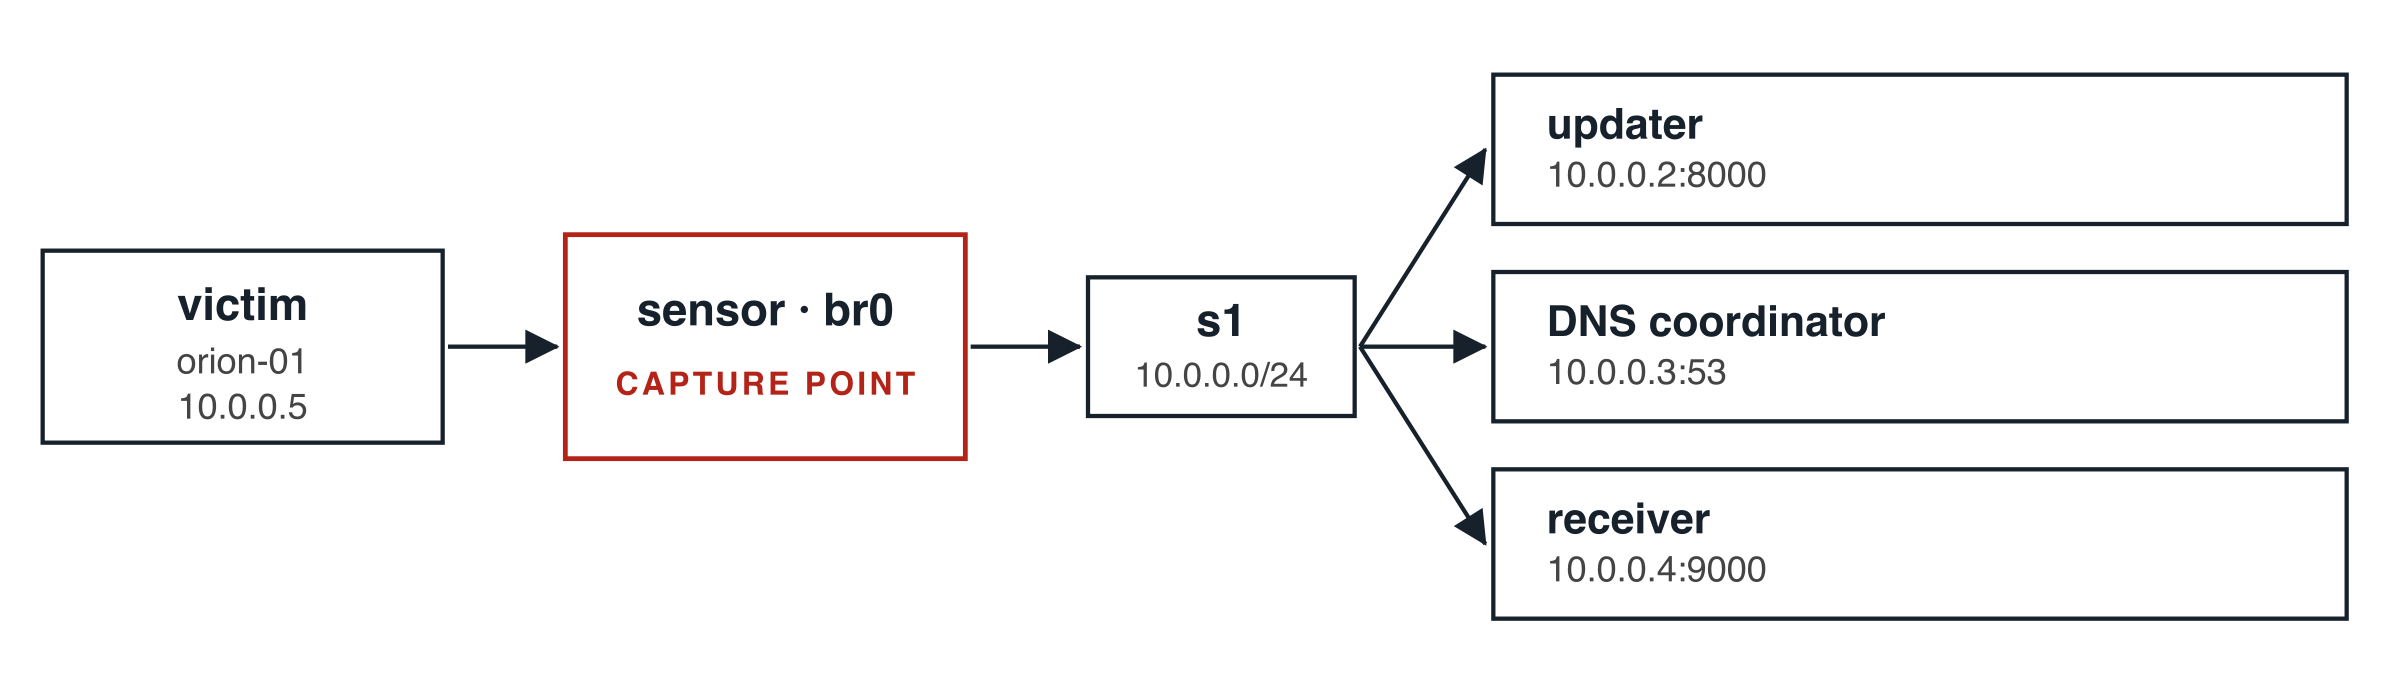
\includegraphics[width=\textwidth]{topology.png}
\caption{Lab topology. The victim reaches the switch only through the bridge, and the capture holds DNS, update and upload traffic on UDP/53, TCP/8000 and TCP/9000.}
\label{fig:topology}
\end{figure}

\subsection{Implemented chain}

Table~\ref{tab:killchain} maps the incident to the lab. The status column records what the demo runs: the release pipeline, the coordinator mode change, and a task from the operator console.

\begin{table}[H]
\centering
\footnotesize
\hyphenpenalty=10000
\caption{Kill-chain mapping. Implemented: the demo runs this step. Reduced: the trust failure is preserved, but not the actor's tooling or scale.}
\label{tab:killchain}
\begin{tabular}{@{}>{\RaggedRight}p{2.3cm}>{\RaggedRight}p{4.7cm}>{\RaggedRight}p{4.7cm}>{\RaggedRight}p{2.5cm}@{}}
\toprule
\textbf{Phase} & \textbf{In the incident} & \textbf{In the lab} & \textbf{Status} \\
\midrule
Reconnaissance & Build pipeline understood before SUNSPOT was written~\cite{crowdstrike-sunspot} & Nothing & Not modelled \\
Weaponization & Source file replaced during the build, original restored~\cite{crowdstrike-sunspot} & Higher public \texttt{orion-compat} replaces the component in the build workspace; the manifest is generated afterwards and records the component's hash & Performed, reduced \\
Delivery & Signed update through the normal channel~\cite{mandiant-campaign} & Signed package published to a stable channel, downloaded over HTTP & Implemented \\
Exploitation & No vulnerability; the customer trusts the signed package & No vulnerability; the client accepts V3 after all checks pass & Not applicable \\
Installation & Backdoored DLL loads inside Orion & Installer registers the component and starts one process per declaration (the manifest declares one) & Implemented, reduced \\
Command and control & DGA check-in, mode by A record, CNAME handoff, OIP-shaped HTTPS & Encoded check-in, mode by coordinator answer, CNAME used for resolution, HTTP to the bare IP & Implemented, reduced \\
Actions on objectives & TEARDROP to Cobalt Strike, AdFind, credential access, SAML forgery & A shell command and a decoy-file read, issued as PoC commands & Implemented, reduced \\
\bottomrule
\end{tabular}
\end{table}

The client accepts the malicious package because every check passes. The package digest matches the catalogue value, the signature verifies against the pinned key, and the component digest matches the SHA-256 the manifest declares. The package is still malicious.

After installation, the component waits three seconds, builds a base32 label from an XORed record holding a version byte, a mode byte, a user identifier, host and user names, and a CRC-16, and queries the coordinator. A bad checksum returns NXDOMAIN. The coordinator answers \texttt{192.0.2.10} for passive, \texttt{192.0.2.20} for selected (shown as ACTIVE), or NXDOMAIN when disabled. The component starts at mode 4, moves to 5 on the activation address, and exits after a final mode-3 check-in when the coordinator is disabled. The coordinator's CNAME is a fixed handoff name, not a DGA-generated record of the kind the real coordinator returned.

Active traffic goes to \texttt{/swip/upd/orion.improvementprogram.asmx} with an \texttt{Orion/2020.2.4} agent string and a body of fields modelled on the Improvement Program, including \texttt{customerId}, \texttt{machineName}, \texttt{userName}, \texttt{osVersion}, \texttt{ipAddress}, and \texttt{processId}. The receiver answers with \texttt{swip.tasks}, and the component returns output in a \texttt{telemetry} block. The demo sends PoC commands from the operator console.

\subsection{What the recreation does not do}

Weaponization is the largest gap. There is no Orion source build and no \texttt{MsBuild.exe} to watch, so SUNSPOT's replacement and restore is not reproduced. The lab's build trusts a public package that outranks the internal one and runs its install hook, which is dependency confusion rather than a source-file swap, and nothing restores an original. The pipeline copies an approved Python source tree and packages it. It does not compile an Orion product. The real incident used SUNSPOT to swap a source file; the lab models dependency confusion. The lab has no Windows host, no signed PE, and no DLL loaded inside a product. Dormancy is compressed from 12 to 14 days to three seconds, and the environment checks are omitted, which makes the lab implant more portable than the original. Check-ins repeat every four seconds against a real minimum of one minute for HTTP and sleeps measured in hours for DNS. The control channel is plain HTTP so the capture can be read, and the implant queries the coordinator directly instead of using the system resolver. It also posts to the address it resolved rather than to the CNAME host, so the lab exercises a bare-IP variant; the real implant used the hostname and required a preceding A record in specific ranges. There is one victim, no persistence, no second stage, and no lateral movement.

Table~\ref{tab:killchain} overstates completeness. The lab reproduces the trust path and the check-in sequence, not the actor's code.
